\section{Implementazione}\label{sec:progettazione}
In quest'ultima sezione si affronteranno le strutture del progetto nello specifico, analizzando i requisiti del progetto e come questi siano stati implementati nel concreto.\\
\newline
Prima di iniziare con la descrizione, si vuole esporre dei punti chiave comuni lungo tutto il progetto. Seguendo la logica del \textit{single-responsibility principle}\footnote{
    Single responsibility principle: principio di progettazione software che afferma che ogni modulo o classe deve essere responsabile di una singola funzionalità.
}, si è strutturata una rete di \texttt{Croquet.Model} che distribuisse ogni funzionalità del dominio ad un modello diverso, in modo da 
tenere separati i compiti e mantenere una gerarchia ordinata e intuitiva.\\
Altro tassello importante è la decisione di non utilizzare ereditarietà, preferendo la composizione in quanto ritenuta più flessibile e meno vincolante. La struttura si può
raffigurare comunque in una relazione padre-figlio in cui però non è il figlio a estendere il padre, bensì il padre a creare e contenere il figlio. Si tenga presente che in questa
valutazione non è stato preso in considerazione l'estensione di tutte le classi da \texttt{Croquet.Model} e \texttt{Croquet.View} in quanto obbligatorio per il funzionamento di Croquet.\\
In ultima istanza si sono create delle classi JavaScript ausiliarie all'architettura di Croquet che fungono da supporto per la gestione dei dati. Queste classi sono state create per 
racchiudere al loro interno le caratteristiche più importanti dei concetti da modellare e quindi facilitare la manutenzione e migliorare la leggibilità del codice.\\

\subsection{Esensione del supporto di base di Croquet}
Si illustreranno ora le classi di base su cui è costruito il progetto, queste sono state introdotte precedentemente nel paragrafo~\ref{sec:design} e comprendono \texttt{BaseModel} e \texttt{BaseView}.\\
Il \texttt{BaseModel} riporta le seguenti \textit{feature}:
\begin{itemize}
    \item \textbf{automatizzazione della parentela}: ogni modello creato con queste classe avrà un riferimento al modello padre;
    \item \textbf{creazione di un log personalizzato}: ogni modello avrà un log personalizzato con il proprio nome, utile per il debug;
    \item \textbf{gestione della distruzione}: ogni modello ascolterà l'evento \textit{`game-over'} avente come \textit{scope} il \textit{session ID} di modo che, in qualunque momento, in qualsiasi
    punto del codice, se il componente valuta che la partita sia terminata, può lanciare questo evento e distruggere tutti i modelli;
    \item \textbf{nuova inizializzazione}: ogni modello disporrà di due metodi da definire, \texttt{\_initialize} che fa le veci del vecchio \texttt{init}, ora utilizzato per il funzionamento
    del \texttt{BaseModel}, e \texttt{\_subscribeAll} in cui vanno inserite tutte le sottoscrizioni che quel modello deve effettuare.
\end{itemize}
Si noti che la separazione tra \texttt{\_initialize} e \texttt{\_subscribeAll} è solo a scopo di leggibilità del codice. Queste funzioni vengono chiamate entrambe all'avvio del modello, per
tanto non risulterebbe un problema se si facesse una sottoscrizione in \texttt{\_intialize} piuttosto che una inizializzazione di variabile in \texttt{\_subscribeAll}.\\
Si riporta il codice della classe \texttt{BaseModel} nel listato~\ref{lst:BaseModel.js}.
\code{BaseModel.js}{Classe \texttt{BaseModel}.}

Prima di procedere con l'elenco delle funzionalità della \texttt{BaseView} si vuole sottolineare che quando si parlerà di molteplici view, non si farà riferimento ad esse in senso
\textit{orizzontale}, ovvero che ogni view contraddistingua un utente diverso, bensì in senso \textit{verticale}, ovvero che ogni utente disponga di più view, ognuna delle quali mostra oggetti diversi (si faccia riferimento alla figura~\ref{fig:MultiViews.png}).\\
\img[0.6]{MultiViews.png}{Visione \textit{verticale} e \textit{orizzontale} delle view a confronto.}
Le feature che presenta la \texttt{BaseView} sono:
\begin{itemize}
    \item \textbf{automatizzazione della parentela}: ogni view creata con questa classe avrà un riferimento alla view padre;
    \item \textbf{automatizzazione del riferimento al model}: ogni vista creata con questa classe avrà un riferimento al model corrispettivo;
    \item \textbf{creazione di un log personalizzato}: ogni view avrà un log personalizzato con il proprio nome, utile per il debug;
    \item \textbf{nuova inizializzazione}: ogni view disporrà di tre metodi da definire, \texttt{\_initialize} che fa le veci del vecchio \texttt{init}, ora utilizzato per il funzionamento
    della \texttt{BaseView}, \texttt{\_subscribeAll} in cui vanno inserite tutte le sottoscrizioni che quella view deve effettuare e \texttt{\_initializeScene} che deve contenere tutte le
    inizializzazioni relative ad oggetti di scena;
    \item \textbf{automatizzazione dell'aggiornamento}: un punto cieco dell'architettura di Croquet è che la chiamata del metodo \texttt{update} non viene perpetrata da una view all'altra.
    Fornendo una lista \texttt{children} riempita con i riferimenti a tutte le view figlie, la \texttt{BaseView} potrà accedere a tutte le viste dalle quali poi richiamare i rispettivi
    \texttt{update} così da sopperire alla mancanza di Croquet. Viene fornito anche un metodo \texttt{\_update} da sovrascrivere per aggiungere funzionalità all'aggiornamento;
    \item \textbf{gestione della distruzione}: ogni view ascolterà l'evento \textit{`game-over'} avente come \textit{scope} il \textit{session ID} di modo che, se venisse lanciato, la view
    si distrugga automaticamente. Per attuare ciò viene lasciata una lista \texttt{sceneObjects} da riempire con tutte le \textit{mesh} di BabylonJS istanziate in modo tale che,
    alla chiamata di distruzione, la \texttt{BaseView} possa distruggere anch'essi. Inoltre, essendo una UI, si è previsto che le view avessero bisogno di un tempo d'attesa prima di 
    cancellare tutta la scena, affinchè ogni oggetto faccia la sua uscita di scena e/o mostri informazioni riguardanti il termine del gioco. Per realizzare ciò si è costruito un metodo 
    da estendere chiamato \texttt{\_endScene} nel quale effettuare tutte le animazioni del caso e che restituisca il numero di millisecondi da aspettare prima di lanciare il comando di 
    \texttt{detach};
    \item \textbf{informazioni condivise}: si è creata una struttura dati che fosse accessibile da tutte le viste e che racchiudesse le informazioni univoche per ogni partita come una sorta
    di \textit{singleton pattern}. Qui si possono trovare informazioni come il riferimento all'\textit{engine} di BabylonJS utilizzato, alla scena o alla telecamera.
\end{itemize}
Si noti che, per quanto possa essere richiamata da qualsiasi punto del codice, la \textit{`game-over'} venga lanciata solo dal modello. Questo perchè, essendo il modello l'unico 
componente che conosce lo stato della partita, è l'unico che può valutare se la partita sia terminata o meno.\\
Anche in questo caso, si lascia il sorgente della classe \texttt{BaseView} nel listato~\ref{lst:BaseView.js}.
\code{BaseView.js}{Classe \texttt{BaseView}.}


\subsection{Visualizzazione degli ologrammi personali e condivisi in tempo reale}
Si definisce ologramma condiviso un ologramma che è visibile da tutti gli utenti connessi alla sessione. Al contrario, un ologramma personale è un oggetto di scena che può essere diverso
da utente a utente e talvolta anche non esserci.\\
Per realizzare un ologramma condiviso basterà creare nella view un oggetto di scena con coordinate assolute. Visto che tutti gli utenti eseguono lo stesso codice, quando
dovranno istanziare l'ologramma condiviso lo faranno tutti allo stesso modo. Per il medesimo motivo, quando il model lancia un evento per comunicare l'aggiornamento dello stato, tutte le 
view lo riceveranno aggiornando l'ologramma alla stessa maniera.\\
Per creare un ologramma personale si è ricorsi all'istanziamento degli oggetti in modo condizionale. Questo significa che, in base a certe condizioni, vengono creati oggetti di scena 
diversi. Nel caso particolare del videogioco, ad esempio, se l'utente è un player ed è il suo turno verrà mostrato un
\textit{near menu}, ovvero un menù capace di seguire l'utente (nativo di MRTK e integrato in BabylonJS), per procedere di fase, al contrario, se non è il suo turno o se non è un
player, non verrà mostrato nulla. Si fornisce il codice~\ref{lst:ologrammi.js} come esempio. Si lasciano anche delle foto dell'applicazione vera e propria in figura~\ref{fig:OlogrammiCondivisi.jpg}
dove vengono mostrati gli ologrammi condivisi dai due giocatori.
\begin{figure}
    \centering

    \begin{subfigure}{0.6\textwidth}
        \centering
        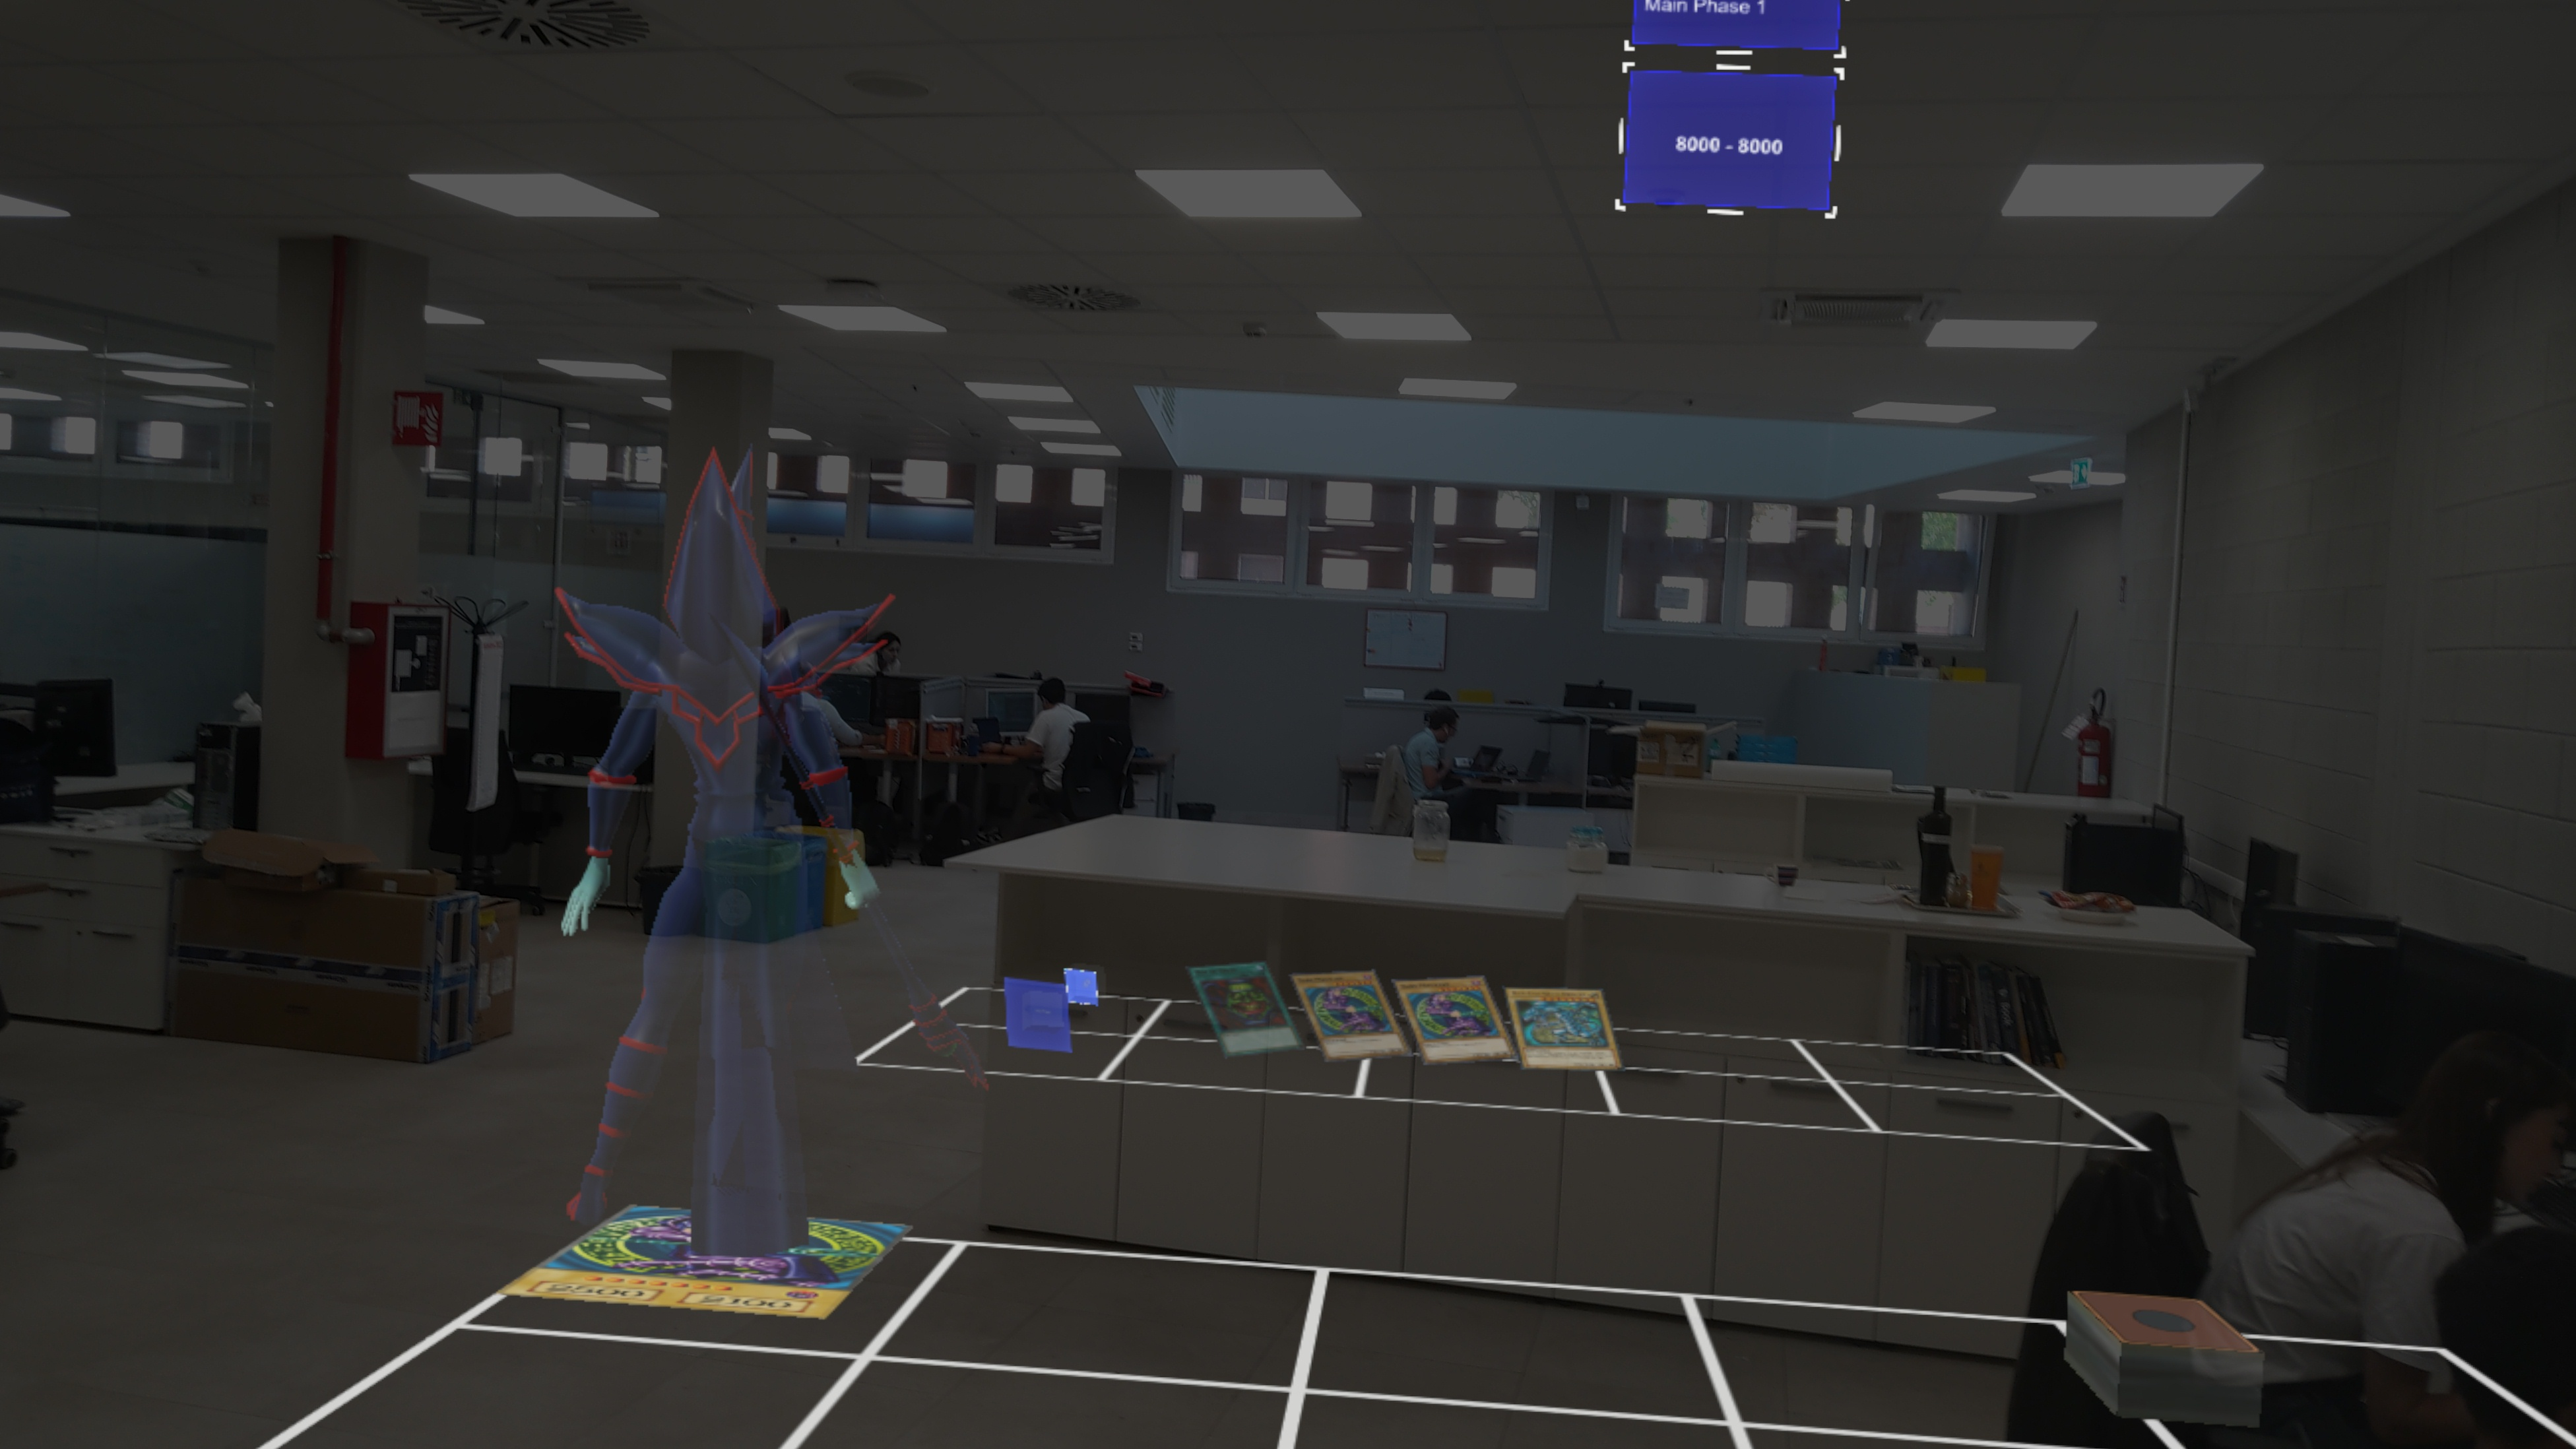
\includegraphics[width=\linewidth]{images/OlogrammiCondivisi1.jpg}
        \caption{Ologrammi condivisi visti dal giocatore uno (che indossa HoloLens).}
        \label{fig:OlogrammiCondivisi1.jpg}
    \end{subfigure}

    \vspace{1cm}

    \begin{subfigure}{0.6\textwidth}
        \centering
        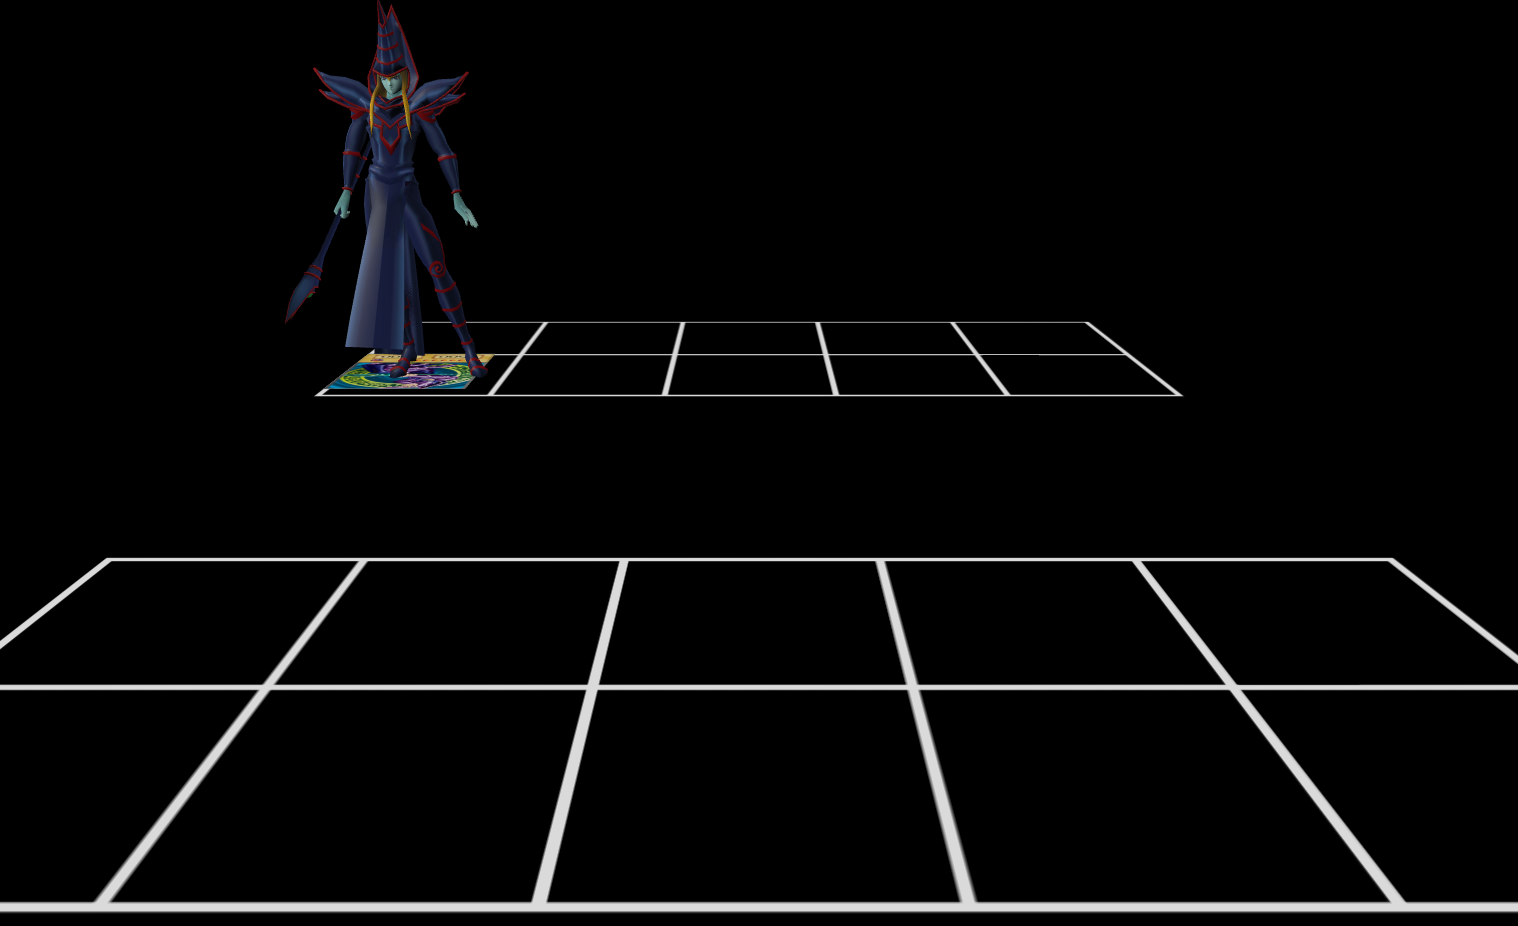
\includegraphics[width=\linewidth]{images/OlogrammiCondivisi2.png}
        \caption{Ologrammi condivisi visti dal giocatore due (che gioca da PC).}
        \label{fig:OlogrammiCondivisi2.jpg}
    \end{subfigure}

    \caption{Ologrammi condivisi visti dai due giocatori.}
    \label{fig:OlogrammiCondivisi.jpg}
\end{figure}
\code{ologrammi.js}{Esempio di istanziazione di ologrammi personali e condivisi.}

\subsection{Interazioni del giocatore}
Per tutte le interazioni del giocatore lungo tutto il corso del progetto si è seguito sempre lo stesso pattern:
\begin{enumerate}
    \item l'utente interagisce con un oggetto di scena;
    \item l'oggetto di scena lancia un evento;
    \item il model riceve l'evento e aggiorna lo stato;
    \item in base a come è costruita la view:
    \begin{enumerate} 
        \item se la view utilizza il metodo \texttt{\_update} per aggiornare la scena, il model non fa nulla;
        \item altrimenti il model lancia un evento per comunicare l'aggiornamento dello stato alla view;
    \end{enumerate} 
    \item la view aggiorna la scena.
\end{enumerate} 
Si prenda d'esempio l'interazione con la mano del giocatore. L'utente interagisce con una carta tra quelle presenti nello spazio personale, la carta lancia un evento \textit{`playCard'}
che viene intercettato del model corrispondente \texttt{HandModel}. Questo verifica che ci siano le condizioni adatte per poter giocare la carta e, se così fosse, aggiorna lo stato
rimuovendo la carta dalla mano e aggiungendola al campo di battaglia. Il model quindi lancia due eventi: uno per rimuovere la carta dalla mano ed uno per aggiungere la carta al
campo di battaglia. La view \texttt{HandView} riceve l'evento \textit{`removeCard'} e rimuove la carta dallo spazio personale, mentre la view \texttt{BattlefieldView} riceve l'evento
\textit{`placeCard'} e crea la carta nel campo di battaglia. Si riporta il codice~\ref{lst:interazioni.js} che illustra quanto detto.
\code{interazioni.js}{Esempio di interazione tra utente e oggetto di scena con conseguente aggiornamento dello stato tramite eventi.}

Per lasciare un esempio anche delle interazioni che coinvolgono l'utilizzo della \texttt{\_udpdate}, si prenda in considerazione l'interazione che l'utente svolge per cambiare la 
fase di gioco. All'utente viene fornito un \textit{near menu} che contiene un pulsante per avanzare di fase. L'utente interagisce con il bottone che lancia un evento 
\textit{`nextPhase'} intercettato dal model \texttt{TurnModel} che aggiorna lo stato. Tornando alla \texttt{TurnView}, nel suo metodo \texttt{\_update}, controlla se lo stato sia
cambiata e, in caso affermativo, aggiorna la scena. Si faccia riferimento al listato~\ref{lst:ologrammi.js} precedentemente mostrato per capire come è stato implementata questa
interazione. Si riporta una schermata dell'applicazione in figura~\ref{fig:InterazioneFase.jpg} dove si può vedere il \textit{near menu} e ciò che avviene dopo essere stato premuto.
\begin{figure}
    \centering

    \begin{subfigure}{0.8\textwidth}
        \centering
        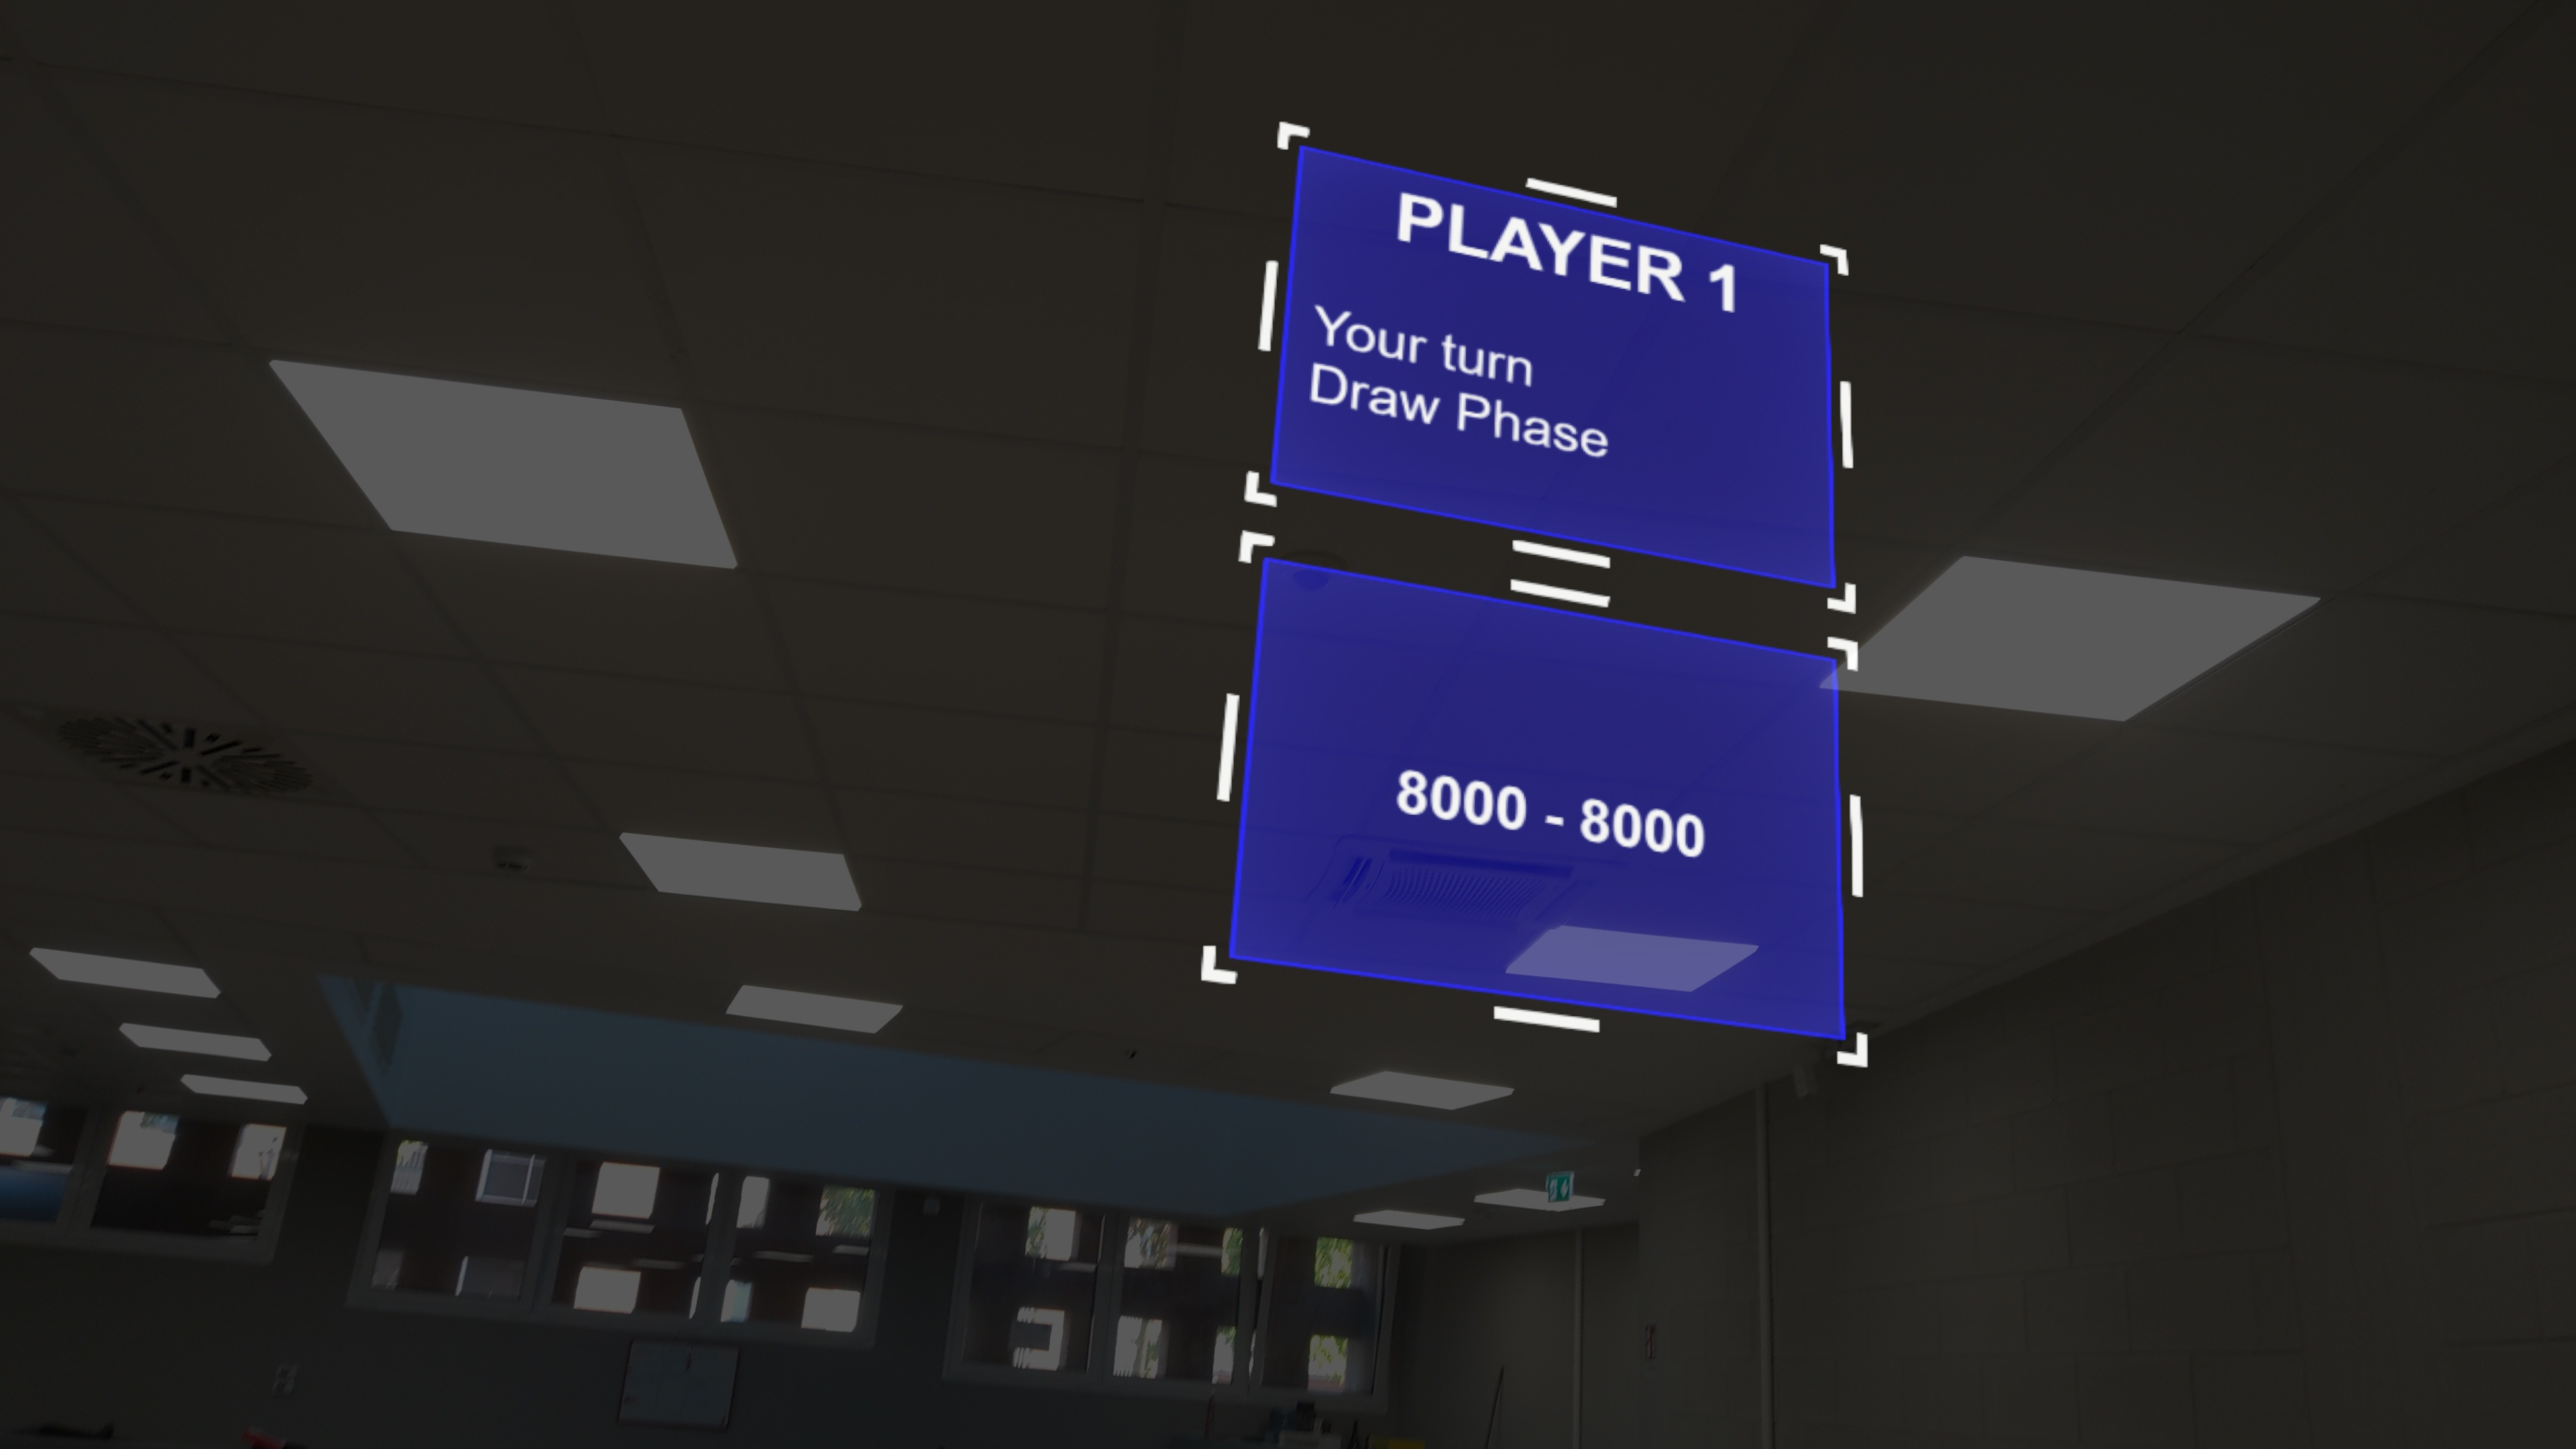
\includegraphics[width=\linewidth]{images/interazione1.jpg}
        \caption{Inizio dell'interazione, stato inziale:\textit{draw phase}.}
        \label{fig:interazione1.jpg}
    \end{subfigure}

    \vspace{1cm} % Spazio verticale tra le due subfigure

    \begin{subfigure}{0.8\textwidth}
        \centering
        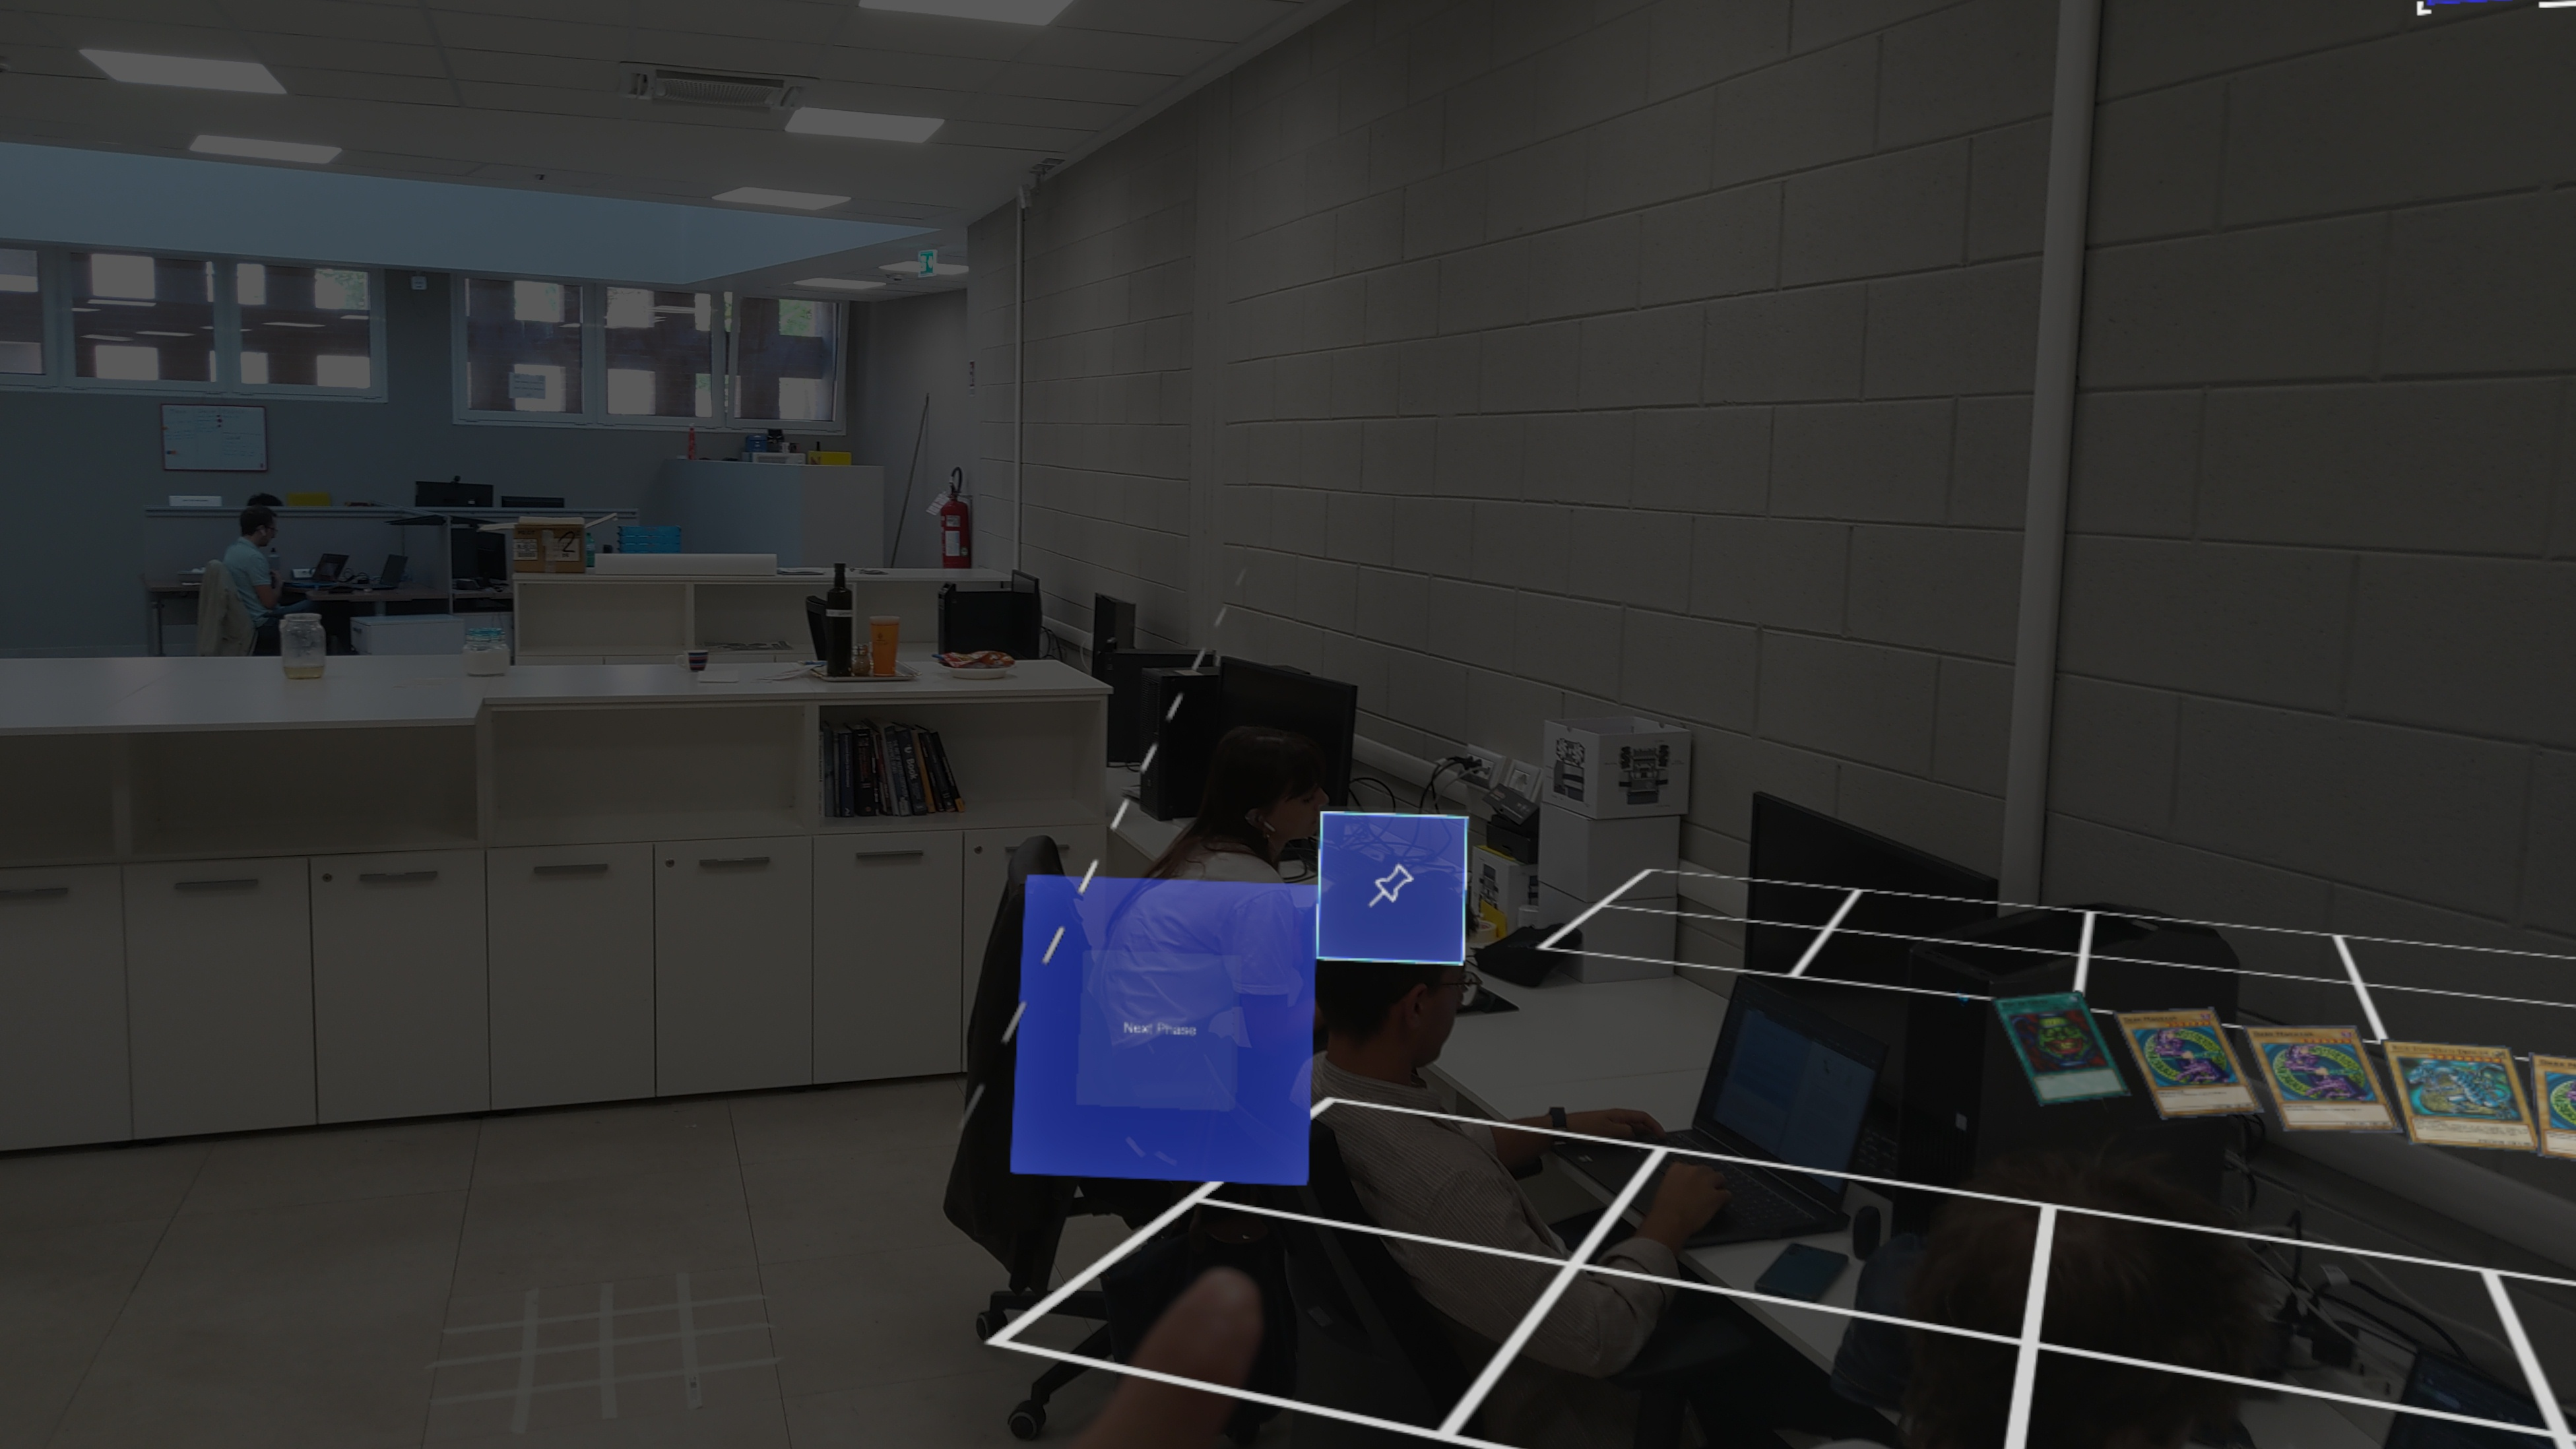
\includegraphics[width=\linewidth]{images/nearMenu.jpg}
        \caption{Pressione del \textit{near menu}.}
        \label{fig:nearMenu.jpg}
    \end{subfigure}

    \vspace{1cm} % Spazio verticale tra le due subfigure

    \begin{subfigure}{0.8\textwidth}
        \centering
        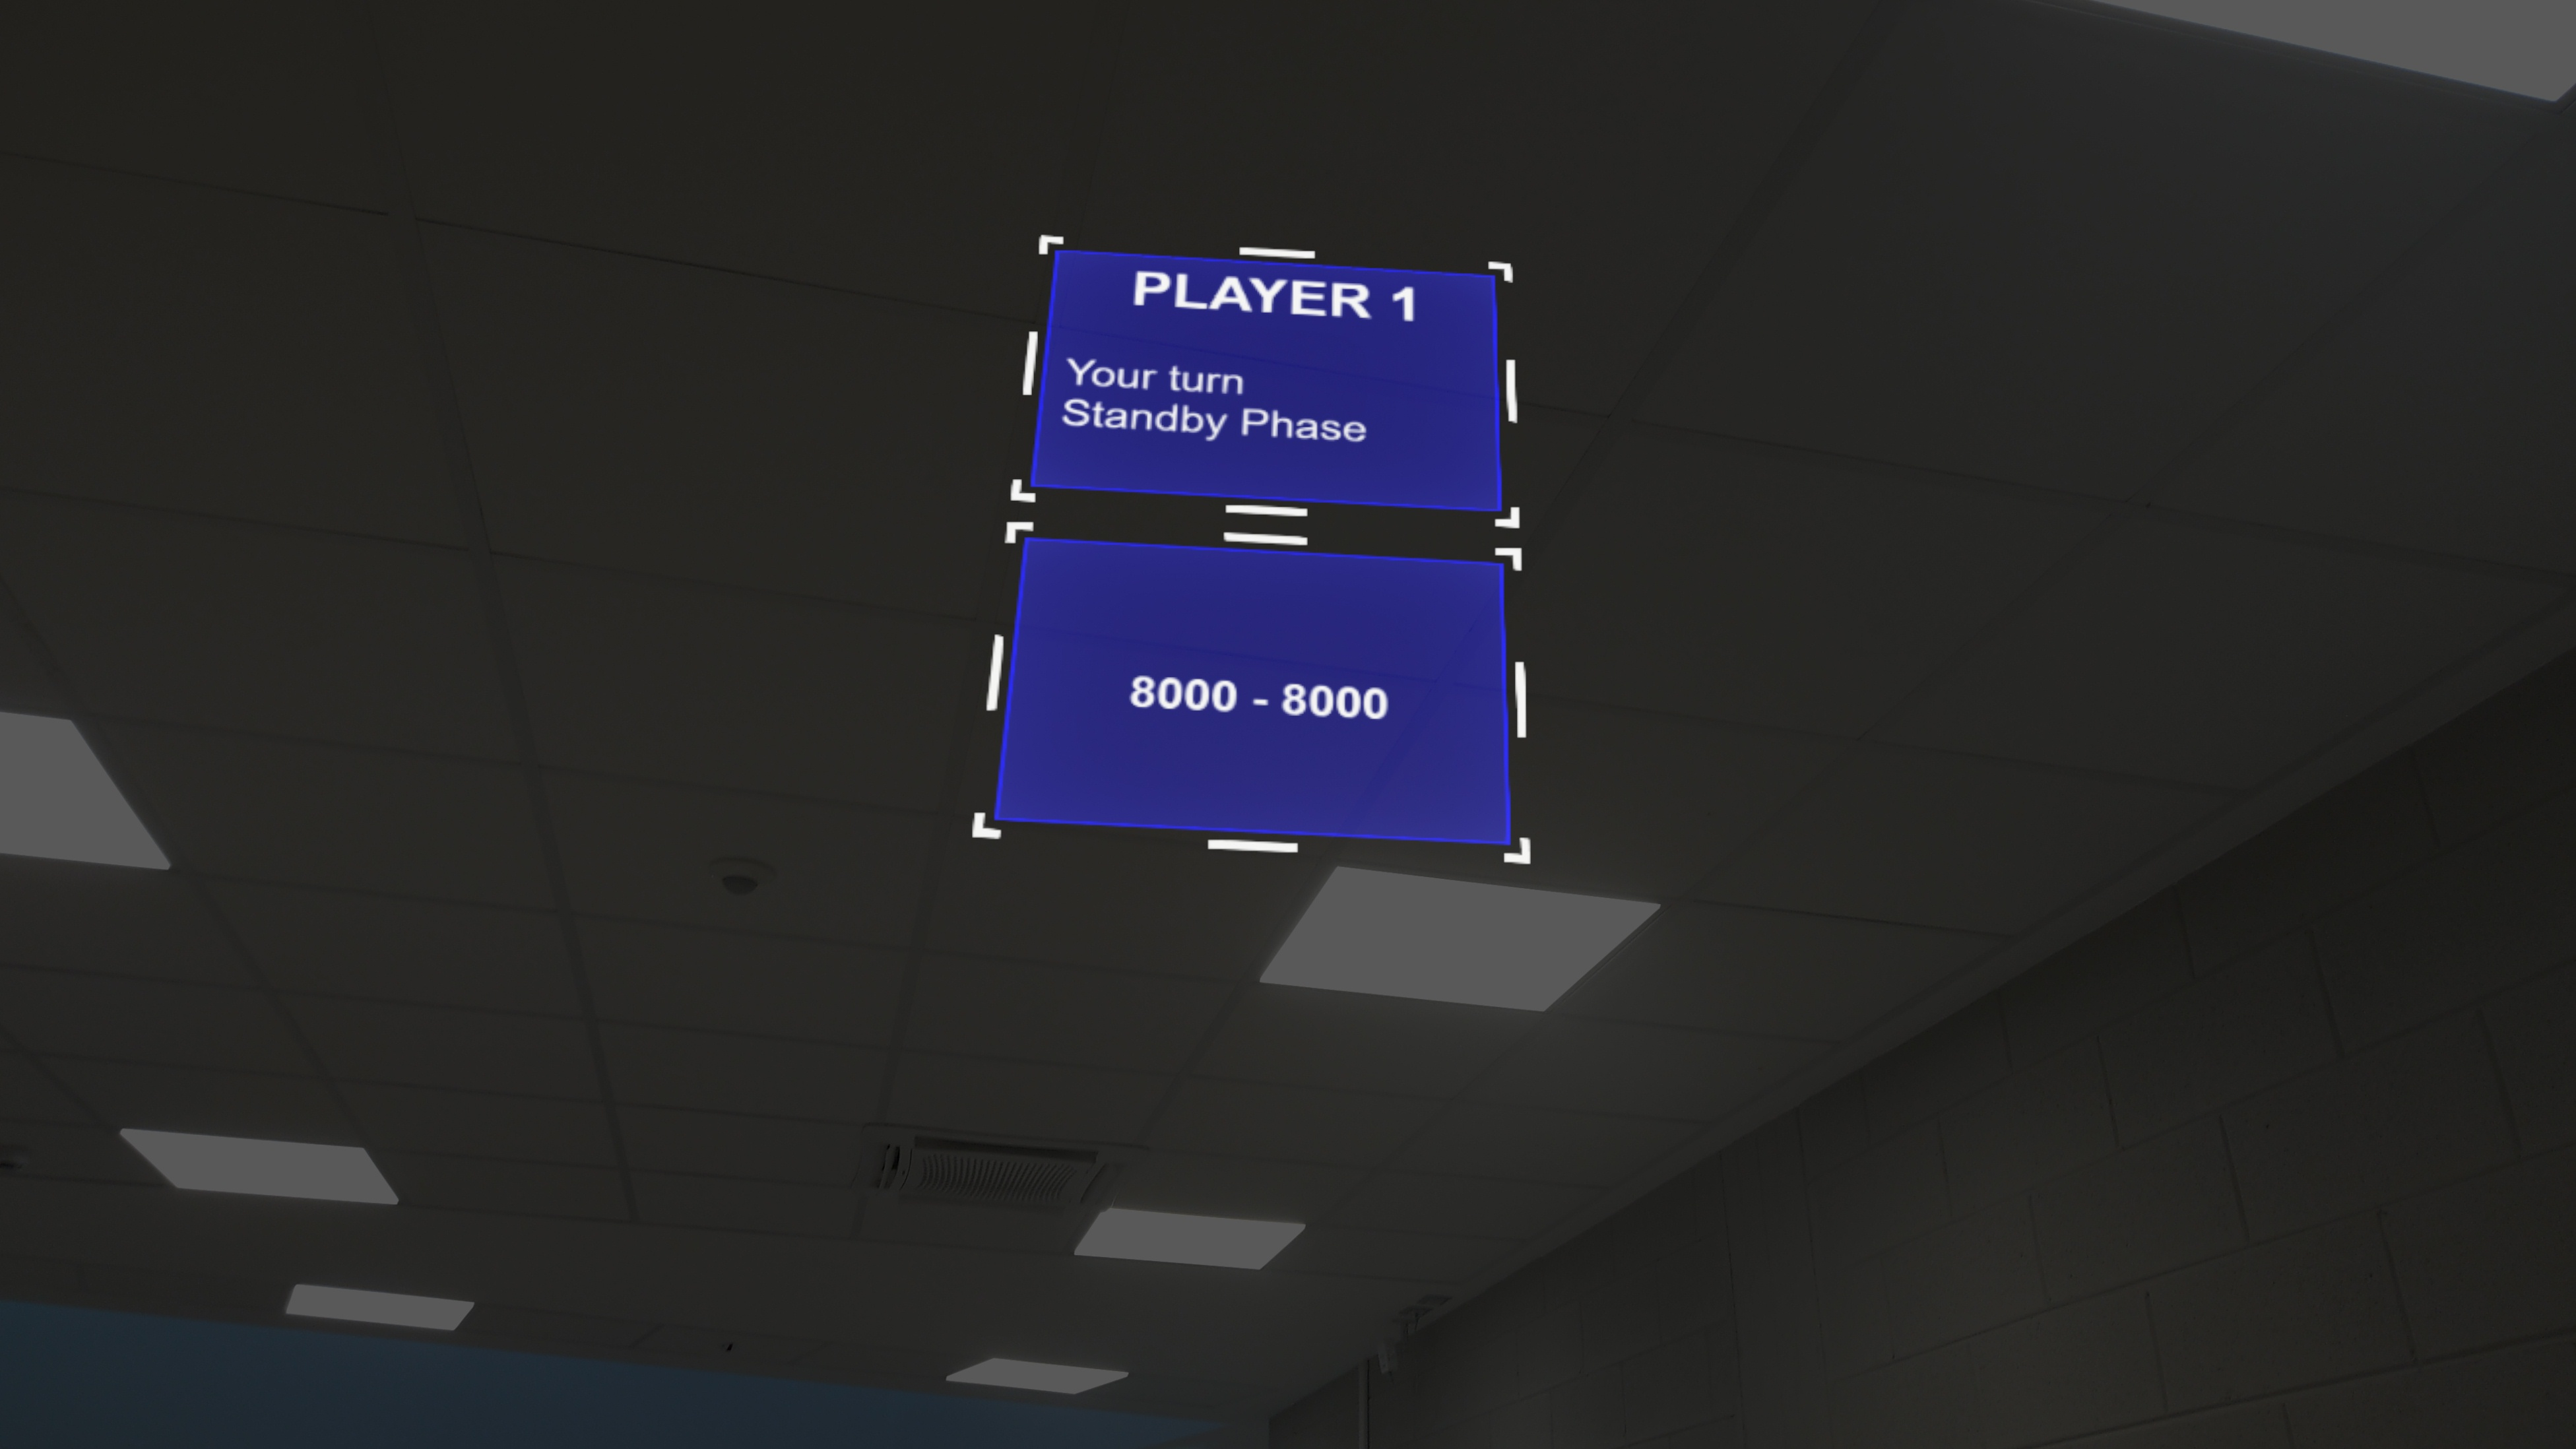
\includegraphics[width=\linewidth]{images/interazione2.jpg}
        \caption{Fine dell'interazione, stato finale: \textit{main phase}.}
        \label{fig:interazione2.jpg}
    \end{subfigure}

    \caption{Fasi dell'interazione tra utente e \textit{near menu}.}
    \label{fig:interazioneFase.jpg}
\end{figure}


\subsection{Gestione delle connessioni}
Nel progetto si è dato un peso rilevante a tutta la parte di gestione delle connessioni e disconnessioni degli utenti. Si sono create infrastrutture apposite che sapessero controllare
e mantenere in uno stato coerente le connessioni di tutti i giocatori.\\
Questo compito lo si è affidato alle classi \texttt{GameModel} e \texttt{GameView}, figlie dirette delle \textit{root classes}, ovvero le prime classi create nel progetto.
Queste classi hanno il compito di gestire le comunicazioni e di istanziare tutti i modelli e le viste del gioco. Si sono dovute gestire tutte le casistiche possibili, come la 
connessione di un nuovo giocatore, la disconnessione temporanea di un giocatore, la riconnessione di un giocatore e la disconnessione definitiva di un giocatore. 
Per dare una panoramica generale di come si è risolto il problema si lascia il codice~\ref{lst:connessioni.js} d'esempio. Nel listato è stata omessa la classe \texttt{GameView} per 
brevità, preferendo una spiegazione discorsiva delle funzionalità.\\
La classe \texttt{GameView} attua tutte le sue logiche attraverso l'utilizzo di quattro eventi diversi.
\begin{itemize}
    \item Ascolta l'evento \textit{`join-response'}: lanciato dopo che il model ha calcolato quale ruolo rappresenti la view appena connessa nella sessione in corso. In base al ruolo
    assegnato, la view istanzierà le view corrispondenti e posizionerà la telecamera dell'utente in modo da avere una visione ottimale della scena.
    \item Ascolta l'evento \textit{`opponent-left'}: lanciato quando un giocatore si disconnette temporaneamente dalla sessione. La view interromperà il normale flusso di gioco, 
    mostrando agli utenti rimasti una schermata d'attesa.
    \item Ascolta l'evento \textit{`opponent-recover'}: lanciato quando un giocatore si riconnette alla sessione. La view farà riprendere la scena da dove era stata interrotta.
    \item Ascolta l'evento \textit{`game-over'}: lanciato quando un giocatore si disconnette definitivamente dalla sessione. La view distruggerà la scena e ricreerà quella di base.
\end{itemize}
\code{connessioni.js}{Infrastruttura per la gestione delle connessioni.}
Un altro aspetto importante che è stato gestito è la possibilità di riavviare la simulazione senza dover ricaricare la pagina. Se tutte le classi si autodistruggessero alla fine del
gioco, l'utente si ritroverebbe con una schermata vuota e dovrebbe ricaricare la pagina per avviare una nuova sessione. Per aggirare il problema si è deciso di cambiare il 
comportamento che hanno le \textit{root classes} al termine della partita, facendo sì che ricreino la scena (e anche i dati) da zero anzichè distruggersi, come mostrato nel 
codice~\ref{lst:root.js}.
\code{root.js}{Creazione e riavvio della simulazione.}

\subsection{Gestione dei dati ed estendibilità}
Si è fatta particolare attenzione anche al trovare un modo per rendere il più facilmente estendible parti critiche del progetto. L'area che necessitava di più attenzione era quella
relativa alle carte da gioco. Si voleva rendere l'aggiunta, la modifica e la rimozione delle carte il più semplice possibile, a tal punto che anche un non programmatore potesse 
metterci mano. Trattandosi di carte collezionabili, ovvero un insieme di carte in continua produzione e sempre diverse, non si poteva pensare ad una struttura dati statica, come si 
farebbe per un normale mazzo di carte francesi. Si è quindi pensato di creare un file JSON che contenesse tutte le informazioni necessarie per creare una carta. Questo file è stato
poi letto e mappato in una struttura dati JavaScript che potesse essere utilizzata dal resto del progetto. Si è scelto di utilizzare un file JSON per la sua semplicità di lettura e
modifica. Anche un non programmatore potrebbe essere in grado, una volta letti i primi esempi presenti nel file, di aggiungere, modificare o rimuovere carte. Si lascia il
file sorgente al listato~\ref{lst:card.json}.
\code{card.json}{Esempio di file JSON contenente le informazioni di carte \textit{Yu-Gi-Oh!}.}